\section{\textit{COCOMO} approach}
\subsection{Source Lines of Code}
\paragraph{}Since we are planning to implement our system through the JEE environment, we use an average conversion factor of 46\footnote{Documented in \url{http://www.qsm.com/resources/function-point-languages-table}}. The \textit{Source Lines of Code} (SLOC) is: $$SLOC = 46 \times 117 = 5382$$

\subsection{Scale Drivers}
The scale drivers considered are\footnote{Taken from \url{http://sunset.usc.edu/research/COCOMOII/Docs/modelman.pdf}}:
\begin{itemize}
\item \textit{Precedentedness} (PREC): describe the previous experience of the organization with this type of project.
\item \textit{Development Flexibility} (FLEX): Degree of flexibility of the development process
\item \textit{Architecture/Risk resolution} (RESL): Extent of risk analysis carried out.
\item \textit{Team cohesion} (TEAM): how the development team know each other and work together
\item \textit{Process maturity} (PMAT): Process maturity of organization dependent on the CMM Maturity Questionnaire.
\end{itemize}
\paragraph{}In the following table\footnote{Taken from: \url{http://sunset.usc.edu/research/COCOMOII/Docs/modelman.pdf}} we describe the meanings of the different values that each scale driver can have.
\begin{figure}[H]
\centering
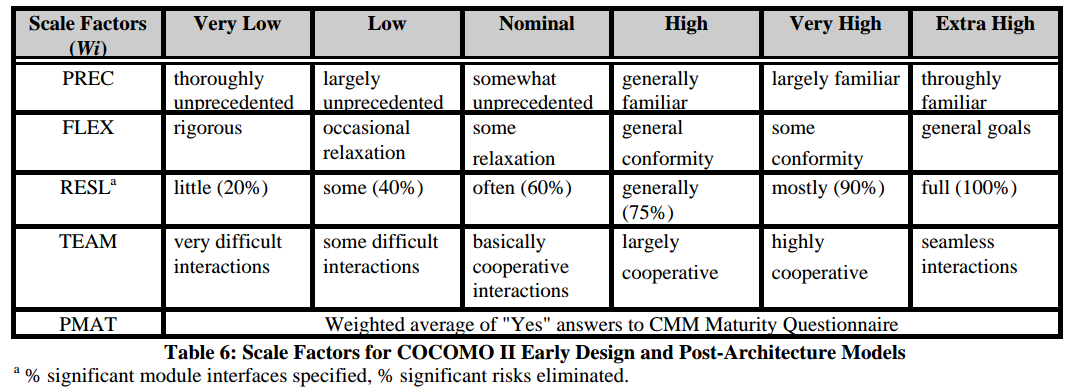
\includegraphics[trim= +70 0 0 0, scale = 0.45]{Size_Cost_Effort/scaleDriversTable}
\caption{Scale drivers levels explanation}
\end{figure}
\paragraph{} In the case of \textit{myTaxiService} the following table describe the choice for each scale driver
\begin{table}[H]
\centering
\begin{tabular}{l | c}
\textbf{Scale driver} & \textbf{Value}\\ \hline
PREC & Very Low \\ \hline
FLEX & High \\ \hline
RESL & Low \\ \hline
TEAM & Nominal \\ \hline
PMAT & Nominal 
\end{tabular}
\caption{Scale drivers values}
\end{table}
\paragraph{} The scale drivers are used in order to calculate the scale exponent E, according to the following formula:
$$E = 0.91 + 0.01 \times \sum_{j = 1}^{5}(SF_j)$$
where the values of $SF_j$ are from the following table
\begin{figure}[H]
\centering
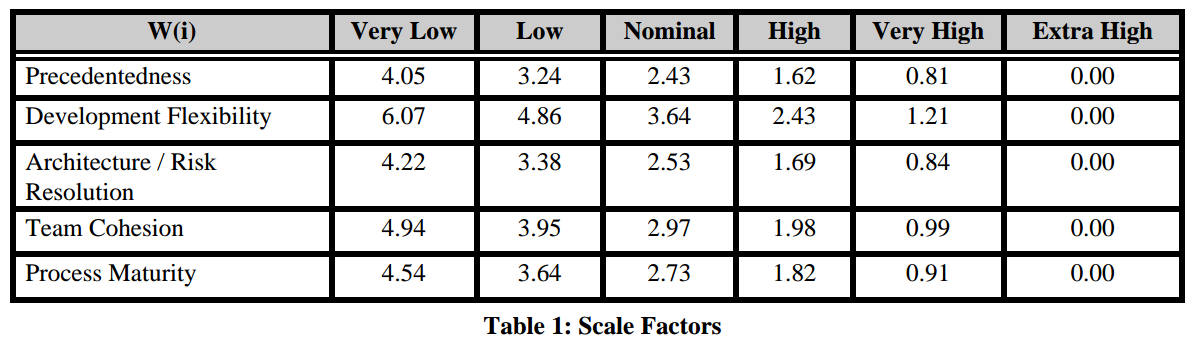
\includegraphics[scale = 0.35]{Size_Cost_Effort/scaleFactors}
\caption{Scale factors}
\end{figure}
\subsection{Cost drivers}
The COCOMO II uses 17 different cost drivers. They are grouped into four categories: \textit{Product, Platform, Personnel} and \textit{Project}.

\begin{table}[H]
\centering
\begin{tabular}{ p{0.25\textwidth} | p{0.75\textwidth}}
\textbf{Product factor} & \textbf{Description} \\ \hline
Required Software Reliability (RELY) & Extent to which the software must perform its intended function over a period of time \\ \hline
Data Base size (DATA) & This measure attempts to capture the affect large data requirements have on product development. \\ \hline
Product Complexity (CPLX) & Control operations, computational operations, device-dependent operations, data management operations, and user interface management operations. \\ \hline
Required Reusability (RUSE) &  Effort needed to construct components intended for reuse on the current or future projects \\ \hline
Documentation match to life-cycle needs (DOCU) & Suitability of the project's documentation to its life-cycle needs
\end{tabular}
\caption{Product cost drivers}
\end{table}

\begin{table}[H]
\centering
\begin{tabular}{p{0.3\textwidth} | p{0.7\textwidth}}
\textbf{Platform factor} & \textbf{Description}\\ \hline 
Execution Time Constraint (TIME) & Execution time constraint imposed upon a software system \\ \hline
Main Storage Constraint (STOR) & Degree of main storage constraint imposed on a software system or subsystem \\ \hline
Platform Volatility (PVOL) & "Platform" is used here to mean the complex of hardware and software (OS, DBMS, etc.) the software product calls on to perform its tasks. It encodes the change of platform over 12 months
\end{tabular}
\caption{Platform cost drivers}
\end{table}

\begin{table}[H]
\centering
\begin{tabular}{p{0.3\textwidth} | p{0.7\textwidth}}
\textbf{Personnel factor} & \textbf{Description}\\ \hline
Analyst Capability (ACAP) & The major attributes that should be considered in this rating are Analysis and Design ability, efficiency and thoroughness, and the ability to communicate and cooperate \\ \hline
Programmer Capability (PCAP) & Evaluation should be based on the capability of the programmers as a team rather than as individuals. \\ \hline
Applications Experience (AEXP) &  The ratings are defined in terms of the project team's equivalent level of experience with this type of application \\ \hline
Platform Experience (PEXP) & Understanding of the platform, both hardware and software \\ \hline
Language and Tool Experience (LTEX) & Measure of the level of programming language and software tool experience of the project team developing the software system or subsystem \\ \hline
Personnel Continuity (PCON) & Project's annual personnel turnover
\end{tabular}
\caption{Personnel cost drivers}
\end{table}

\begin{table}[H]
\centering
\begin{tabular}{p{0.3\textwidth} | p{0.7\textwidth}}
\textbf{Project factor} & \textbf{Description}\\ \hline
Use of Software Tools (TOOL) & The tool rating ranges from simple edit and code, very low, to integrated lifecycle management tools, very high\\ \hline
Multisite Development (SITE) & Ability of distributed software development \\ \hline
Required Development Schedule (SCED) & Measures the schedule constraint imposed on the project team developing the software
\end{tabular}
\caption{Project cost drivers}
\end{table}

\paragraph{} These cost drivers are evaluated through the following table\footnote{Taken from \url{http://sunset.usc.edu/research/COCOMOII/Docs/modelman.pdf}}

\begin{figure}[H]
\centering
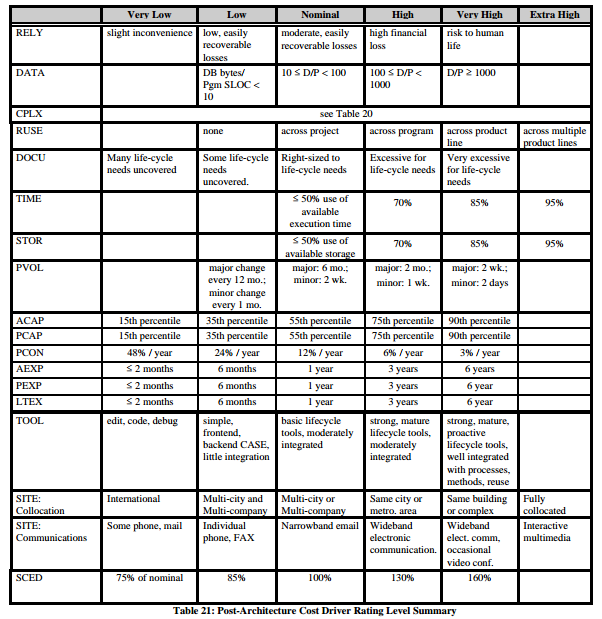
\includegraphics[trim = +40 0 0 0,scale=0.8]{Size_Cost_Effort/costDriversTable}
\caption{Cost drivers levels explanation}
\end{figure}

\paragraph{}In the case of \textit{myTaxiService} are used the following values:
\begin{table}[H]
\centering
\begin{tabular}{l | c}
\textbf{Cost driver} & \textbf{Value} \\ \hline
RELY & Nominal\\ \hline
DATA & Nominal\\ \hline
CPLX & Nominal\\ \hline
RUSE & High\\ \hline
DOCU & High\\ \hline \hline
TIME & Nominal \\ \hline
STOR & High \\ \hline
PVOL & Nominal \\ \hline \hline
ACAP & High \\ \hline
PCAP & High \\ \hline
AEXP & Low \\ \hline
PEXP & Low \\ \hline
LTEX & High \\ \hline
PCON & Very High \\ \hline \hline
TOOL & High \\ \hline
SITE & Low \\ \hline
SCED & High
\end{tabular}
\caption{Values of cost drivers}
\end{table}

\paragraph{} We use this values in order to calculate the \textit{effort adjustment factor} (EAF) like this:
$$EAF = \prod_{j=1}^{17}EM_j$$ where $EM_j$ are the cost drivers factors derived from the following table:
\begin{figure}[H]
\centering
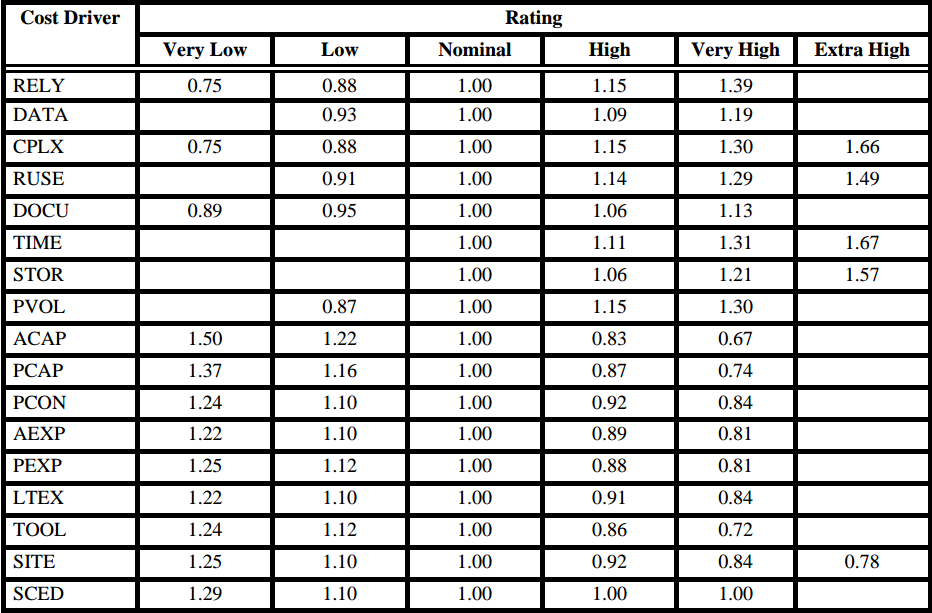
\includegraphics[trim = 50 0 0 0,scale=0.5]{Size_Cost_Effort/costFactors}
\caption{Cost drivers factors}
\end{figure}

\subsection{Effort calculation}
The \textit{effort} (calculated in Person-Months) required is given by the following formula:
$$Effort = 2.94 \times EAF \times \left(\frac{SLOC}{1000}\right)^E$$
And in the particular case of \textit{myTaxiService} it is estimated to be:$$Effort_{myTaxiService} = 15.9 \mbox{ Person-Months }$$

\subsection{Scheduling}
The COCOMO II scheduling equation predicts the number of months required to complete a software project, and consists in the following formula:
$$Duration = 3.67 \times (Effort)^{SE}$$ $$SE = 0.28 + 0.2 \times (E - 0.91)$$
In the case of \textit{myTaxiService} we estimate $$Duration_{myTaxiService} = 11.9 \mbox{ Months }$$

\subsection{Dimensioning of the team}
Finally we compute how big should be the development team for the project. $$People = \frac{Effort}{Duration}$$ and in the specific case of \textit{myTaxiService} we have $$People_{myTaxiService} = 1.36 \approx 2$$

\subsection{Resume}
\begin{figure}[H]
\centering
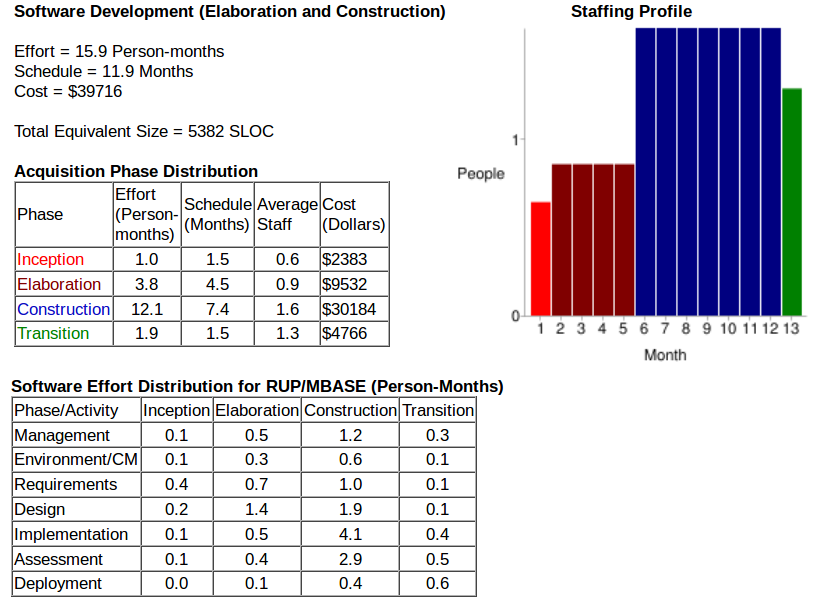
\includegraphics[trim = 60 0 0 0,scale = 0.6]{Size_Cost_Effort/online}
\caption{Resume}
\end{figure}

We supposed to pay our developers an average of 2500\$ per month.